\documentclass[a4paper,10pt]{article}

\usepackage[ngerman]{babel}
% \usepackage[utf8]{inputenc} 
% \usepackage[T1]{fontenc}
% \usepackage[paperwidth=210mm, paperheight=297mm, textheight=240mm, left=2.1cm, right=2.1cm]{geometry}

\usepackage{fontspec}
\setmainfont{playfair.otf}
\setsansfont{montserrat.otf}
\setmonofont{PoliticsHead.otf}
\usepackage{graphicx}
\usepackage{microtype}
\usepackage{enumitem}
\setlist[itemize]{leftmargin=*}

\usepackage{calc}
\newlength{\lmargin}
\setlength{\lmargin}{1in + \hoffset + \oddsidemargin}

\usepackage{flowfram}
\usepackage{color}
\usepackage{tikz}
\setlength{\parindent}{0pt}

% erste Seite
\newflowframe[1]{8cm}{36\baselineskip}{-2.5cm}{-6\baselineskip}[frame1-1a]
\newflowframe[1]{8cm}{36\baselineskip}{7cm}{-6\baselineskip}[frame1-2b]
% % \newflowframe[1]{5cm}{27\baselineskip}{11cm}{0\baselineskip}[frame1-3c]


% definicja ramek typu flow na kolejnych stronach
\newflowframe[2-4]{8cm}{72\baselineskip}{-2.5cm}{-6\baselineskip}[frame2-1a]
\newflowframe[2-4]{8cm}{72\baselineskip}{7cm}{-6\baselineskip}[frame2-2a]
% \newflowframe[>1]{5cm}{57\baselineskip}{11cm}{0\baselineskip}[frame2-3a]

\newflowframe[5]{8cm}{36\baselineskip}{-2.5cm}{-6\baselineskip}[frame5-1a]
\newflowframe[5]{8cm}{36\baselineskip}{7cm}{-6\baselineskip}[frame5-2b]

\newflowframe[6-12]{8cm}{72\baselineskip}{-2.5cm}{-6\baselineskip}[frame6-1a]
\newflowframe[6-12]{8cm}{72\baselineskip}{7cm}{-6\baselineskip}[frame6-2a]

\newflowframe[13]{8cm}{36\baselineskip}{-2.5cm}{-6\baselineskip}[frame13-1a]
\newflowframe[13]{8cm}{36\baselineskip}{7cm}{-6\baselineskip}[frame13-2b]


\newflowframe[14-17]{8cm}{72\baselineskip}{-2.5cm}{-6\baselineskip}[frame14-1a]
\newflowframe[14-17]{8cm}{72\baselineskip}{7cm}{-6\baselineskip}[frame14-2a]


% \newflowframe[16]{8cm}{36\baselineskip}{-2.5cm}{-6\baselineskip}[frame16-1a]
% \newflowframe[16]{8cm}{36\baselineskip}{7cm}{-6\baselineskip}[frame16-2b]
% 
% 
% \newflowframe[17]{8cm}{72\baselineskip}{-2.5cm}{-6\baselineskip}[frame17-1a]
% \newflowframe[17]{8cm}{72\baselineskip}{7cm}{-6\baselineskip}[frame17-2a]

% 
% %definicja ramek statycznych wstawianych na stronie 1
% % frames für bilder
\newstaticframe[1]{\paperwidth}{14cm}{-\lmargin}{12.5cm}[frameS-1a]
\newstaticframe[1]{14cm}{7\baselineskip}{0cm}{45\baselineskip}[frameS-1b]

\newstaticframe[5]{\paperwidth}{14cm}{-\lmargin}{12.5cm}[frameS-5a]
\newstaticframe[5]{14cm}{7\baselineskip}{0cm}{45\baselineskip}[frameS-5b]

\newstaticframe[13]{\paperwidth}{14cm}{-\lmargin}{12.5cm}[frameS-13a]
\newstaticframe[13]{14cm}{7\baselineskip}{0cm}{45\baselineskip}[frameS-13b]

% \newstaticframe[16]{\paperwidth}{14cm}{-\lmargin}{12.5cm}[frameS-16a]
% \newstaticframe[16]{14cm}{7\baselineskip}{0cm}{45\baselineskip}[frameS-16b]


% \newstaticframe[17]{\paperwidth}{14cm}{-\lmargin}{12.5cm}[frameS-17a]
% \newstaticframe[17]{14cm}{7\baselineskip}{0cm}{45\baselineskip}[frameS-17b]


% Seitenzahlen
%definicja ramki dymamicznej wstawiania na stonie nieparzystej
\newdynamicframe[odd]{2cm}{2cm}{-\lmargin}{6cm}[frameD-1a]
%definicja ramki dymamicznej wstawiania na stonie parzystej
\newdynamicframe[even]{2cm}{2cm}{15.1cm}{6cm}[frameD-1b]

% \definecolor{green}{rgb}{0.6,0.8,0.1}

\title{Wahlprogramm Friedrichshain-Kreuzberg -- Piratenpartei}
\author{Piratenpartei Friedrichshain-Kreuzberg}
\date{\relax}

\newcommand{\mysection}[1]{{\vspace{1cm}\noindent\color{gray}{\ttfamily\LARGE\raggedright #1}\\\medskip}}

\newcommand{\abschnitt}[2]{%
\mysection{\raggedright #1}%
\begin{figure}[t]%
\vspace*{-2.7cm}%
\hspace*{-2.1cm}%
% \vspace*{-1.7cm}%
% \hspace*{-1.3cm}%
\includegraphics[width=10cm]{images/blog/large/#2} %
\end{figure}%
}


% \newcommand{\abschnitt}[2]{%
% \mysection{\raggedright #1}%
% \begin{figure}[t]%
% \vspace*{-2.7cm}%
% \hspace*{-2.1cm}%
% % \vspace*{-1.7cm}%
% % \hspace*{-1.3cm}%
% \includegraphics[width=11cm]{images/blog/large/#2} %
% \end{figure}%
% }

\newcommand{\bottomfigure}[1]{
% \begin{figure}
% \\
% \bigskip
\parbox{5cm}{
% \hspace*{-2.1cm}%
\vspace*{1cm}%
\includegraphics[width=10cm]{./images/blog/large/#1}
}
% \end{figure}
% \clearpage
}


\newcommand{\flachmann}[1]{
\begin{figure}[b!]
\\
% \bigskip
\parbox{5cm}{
\hspace*{-7cm}%
\vspace*{1cm}%
\includegraphics[width=20cm]{./images/blog/large/#1}
}
\end{figure}
% \clearpage
}

\newcommand{\querschlaeger}[1]{
\begin{figure}[t]%
\vspace*{-2.7cm}%
\hspace*{-2.1cm}%
\includegraphics[width=\paperwidth]{images/blog/large/#1} %
\end{figure}%
}

\newcommand{\p}{\raisebox{-.5cm}{~}}

\begin{document}
\pagestyle{empty}
\sloppy 

% wstawienie numerów stron w ramki dynamiczne frameD-1a i frameD-1b
\begin{dynamiccontents*}{frameD-1a}
\begin{tikzpicture}
\draw(0,0) node [fill=orange, minimum width=1.5cm, minimum height=1.5cm]{
{\sffamily\bfseries\Huge\color{white}\thepage}
};
\end{tikzpicture}
\end{dynamiccontents*}

\begin{dynamiccontents*}{frameD-1b}
\begin{tikzpicture}
\draw(0,0) node [fill=orange, minimum width=1.5cm, minimum height=1.5cm]{
{\sffamily\bfseries\Huge\color{white}\thepage}
};
\end{tikzpicture}
\end{dynamiccontents*}


% wstawienie grafiki w ramkię statyczną frameS-1a
\begin{staticcontents*}{frameS-1a}

\includegraphics[viewport = {0cm 0cm 21cm 16cm}, clip]{images/blog/large/niemandistnormal.jpg}
\end{staticcontents*}

\begin{staticcontents*}{frameS-5b}
\hspace*{-4.5cm}
\vspace*{2cm}

\includegraphics[width=\paperwidth]{images/blog/large/gruenebetonmischer.png}
\vspace*{1cm}
\end{staticcontents*}



\begin{staticcontents*}{frameS-13a}

\includegraphics[viewport = {0cm 0cm 21cm 16cm}, clip]{images/blog/large/machtlack.jpg}
\end{staticcontents*}

% \begin{staticcontents*}{frameS-16a}
% % \hspace*{-4.5cm}
% \vspace*{2cm}
% 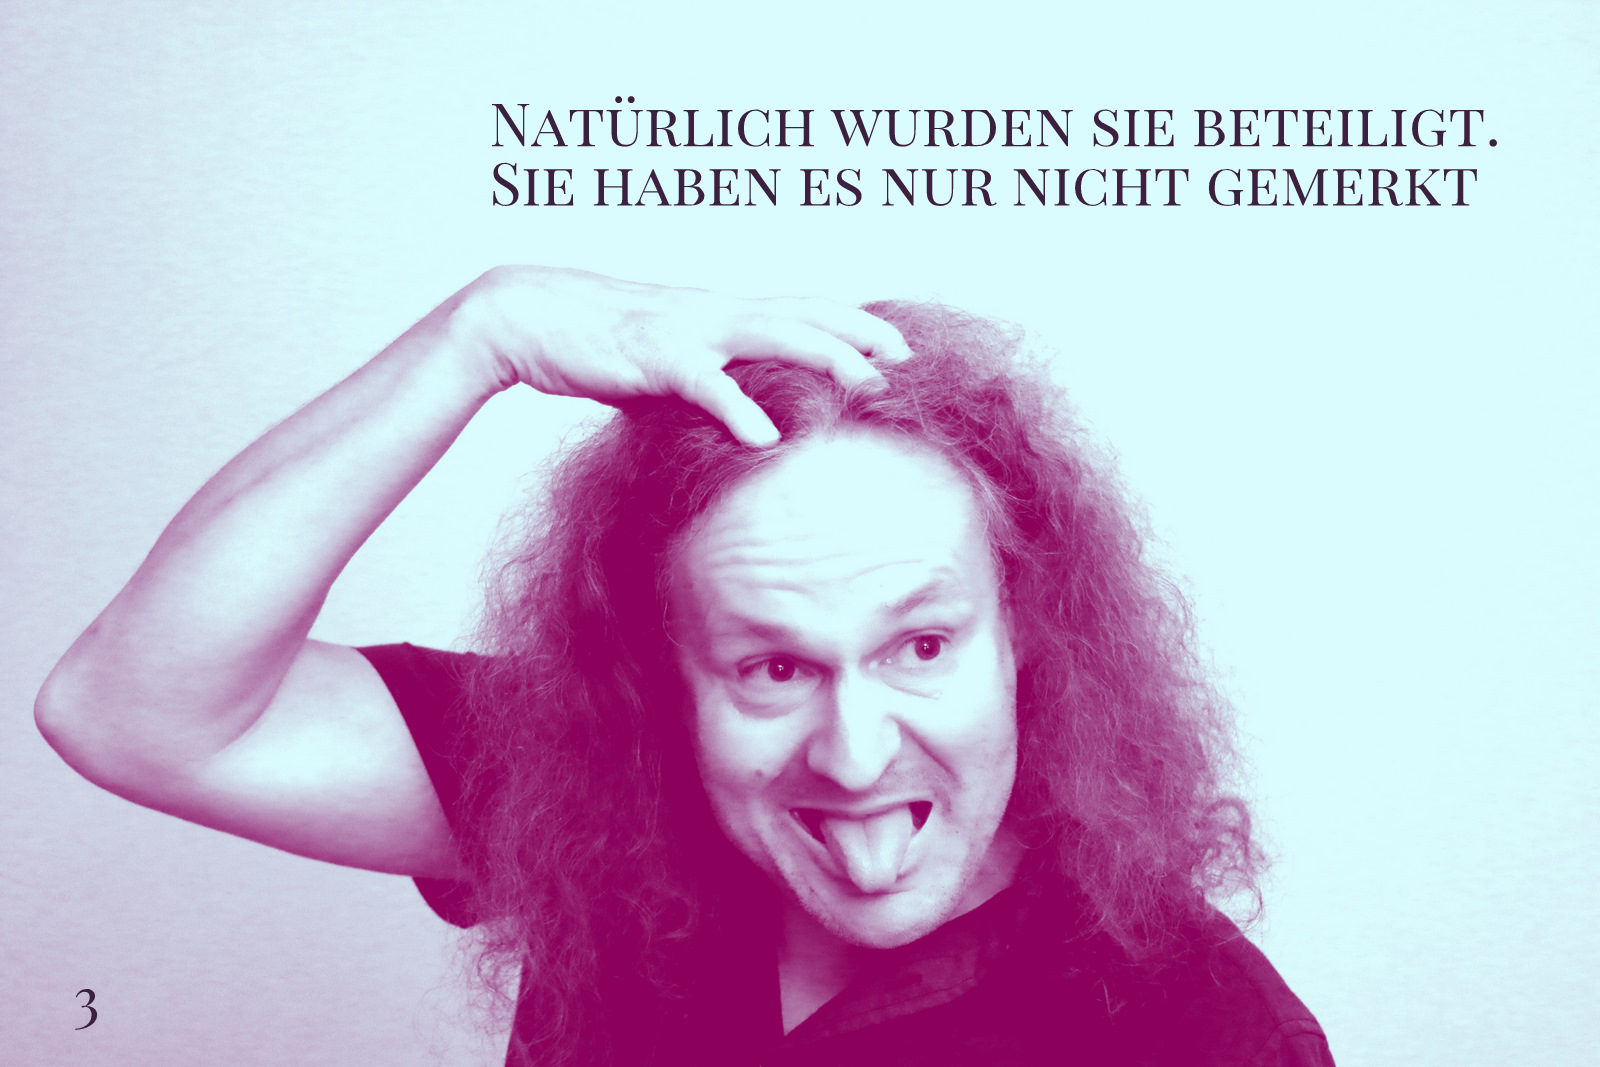
\includegraphics[width=\paperwidth]{images/blog/large/natuerlichwurdensiebeteiligt.jpg}
% \vspace*{1cm}
% \end{staticcontents*}


% \begin{staticcontents*}{frameS-17b}
% % \hspace*{-4.5cm}
% \vspace*{2cm}
% \includegraphics[width=\paperwidth]{images/blog/large/fraktionplus.jpg}
% \vspace*{1cm}
% \end{staticcontents*}



% % wypełnienie tekstem ramki statycznej frameS-1b
% \begin{staticcontents*}{frameS-1b}
% \begin{tikzpicture}
% \draw(0,0) node [fill=white, text width=13cm, inner sep=5mm, opacity=0.7]{
% \large\sffamily 
% \chapter*{Präambel}
% };
% \end{tikzpicture}
% \end{staticcontents*}


% \begin{figure}[t]%
% \vspace*{-2.7cm}%
% \hspace*{-3.3cm}%
% 
\includegraphics[width=\paperwidth]{images/blog/large/niemandistnormal.jpg} %
% \end{figure}%


\mysection{Präambel}%



In Xhain wohnen viele Menschen zusammen und gestalten gemeinsam den
Bezirk. Wir wollen, dass jede*r einzelne sich so gut wie möglich
einbringen kann. Dazu gehört, dass allen Menschen die notwendigen
Informationen zur Verfügung stehen. Daher setzen wir uns für die freie
Zugänglichkeit von Verwaltungsdaten ein. Außerdem sollen alle Ausschüsse
öffentlich sein und die Sitzungen der BVV im Internet live übertragen
werden. Interessenkonflikte von Verordneten sollen in einem
Lobbyregister einsehbar sein.

\enlargethispage{1em}
Die Teilhabe gilt für alle. Wir sind dafür, allen Menschen im Bezirk
unabhängig von Alter oder Staatsangehörigkeit maximale Mitspracherechte
bei der Gestaltung des Bezirks einzuräumen. Auch den Menschen, die
aufgrund der Krise im Nahen Osten und anderen Weltgegenden ganz neu im
Bezirk eingetroffen sind, möchten wir Teilhabe ermöglichen. Dazu gehören
eine menschenwürdige Unterbringung, das Recht auf Freizügigkeit und
Arbeit, Sprachkurse und eine gesellschaftliche Vertretung. Dabei stehen
uns derzeit noch einige Bundesgesetze im Weg, die die Teilhabe, z.B. im
Wahlrecht, unnötig beschränken. Hier gibt es für uns nur eine Richtung:
die der Demokratisierung.Teilhabe wird aber derzeit nicht nur durch
Bundesgesetze beschränkt. 
Wer sich keinen Internetanschluss leisten
kann, kommt u.U. nicht an die notwendigen Informationen und kann sich
nicht vernetzen. Daher fördern wir Freifunk. Mit Freifunk schalten
Menschen ihre Internetanschlüsse zusammen und stellen sie anderen
Menschen zur Verfügung. Zudem ist Freifunk dezentral aufgebaut und
erschwert die staatliche Kontrolle von Kommunikation. Denn wer sich
überwacht fühlt, kommuniziert nicht frei. Daher setzen wir uns auch
gegen die Funkzellenabfragen, gegen massenhafte Videoüberwachung und
gegen geheime Gefahrengebiete im Land ein.Teilhabe wird auch beschränkt
durch mangelnde Mobilität. 
\enlargethispage{1em}
Wer sich kein BVG-Ticket leisten kann, um zur
Ausschusssitzung zu fahren, kann seine Rechte dort nicht vertreten.
Daher treten wir für umlagefinanzierten fahrscheinlosen öffentlichen
Nahverkehr ein. Ein Nebeneffekt wäre die Abschaffung von BVG-Kontrollen
und mehr Platz in den Berliner Justizvollzugsanstalten. Dort sitzen
derzeit viele arme Leute, die sich die in der Stadt notwendige Mobilität
schlicht nicht leisten konnten. Das öffentliche Straßenland soll
ebenfalls allen zur Verfügung stehen. Wir setzen uns für
gleichberechtigte Nutzung des Verkehrsraumes durch alle
Fortbewegungsmittel (zu Fuß, Fahrrad, Auto, Bus, Bahnen) ein. Dabei ist
der gegenseitige Respekt die oberste Prämisse. In diesem Kontext wollen
wir das Konzept Shared Space noch stärker erproben. Auch öffentliche
Grünflächen und Wasserflächen sollen allen Menschen zugänglich sein. Wir
wenden uns gegen die Privatisierung des Spreeufers und das Zubauen von
Brachflächen.

\abschnitt{}{plakat_katze.png}

Durch die Digitalisierung hat sich die Arbeitswelt verändert. Viele
manuelle Tätigkeiten werden heute von Maschinen erledigt. Dies gibt
Menschen mehr Zeit, sich um andere Dinge zu kümmern. Wir begrüßen diese
Automatisierung, stellen aber fest, dass die so gewonnene Zeit nur
wenigen Menschen zugute kommt. Viele Menschen müssen weiter in prekären
Verhältnissen arbeiten und finden keine Arbeit, da Maschinen ihre
Arbeitsplätze wegrationalisiert haben. Daher setzen wir uns für eine
gerechtere Verteilung der Automatisierungsdividende unter allen Menschen
ein. Dies heißt für uns: Bedingungsloses Grundeinkommen.Auch im
täglichen Arbeitsleben gilt für uns das Gebot der Teilhabe. Wir setzen
uns für die Weiterverwendung und gemeinsame Entwicklung von Computercode
ein (Open Source). Auch Büroräume und Infrastruktur können gemeinsam
genutzt werden in sogenannten Coworking Spaces. Menschen sind soziale
Wesen und helfen einander, wenn man ihnen die Möglichkeit dazu gibt.
Dies gilt auch im kulturellen Bereich. Die menschliche Kreativität
findet sich nicht nur in den klassischen Gebäuden der Privilegierten wie
Opernhäusern, sondern auch im viel kleineren Raum, z.B. Jam Sessions
oder Street Art. Wir setzen uns für den Erhalt von nicht-kommerziellen
Freiflächen für Subkultur ein.

\enlargethispage{-3em}
Auch Spiritualität gehört zur menschlichen Kultur und zur menschlichen
Entfaltung. Dabei gilt für uns aber, dass der Staat sich in diesem
Bereich weltanschaulich neutral verhält. Das heißt: keine positive
Diskriminierung von Religionsgemeinschaften durch staatliche
Unterstützung; keine negative Diskriminierung von Religiösen im
Arbeitsmarkt und anderswo.In allen menschlichen Kulturen gibt es Formen
der Berauschung. Einige davon sind gesellschaftlich anerkannt (Alkohol),
andere nicht (Cannabis). Wir setzen uns für eine Dekriminalisierung
aller Drogen bei gleichzeitiger Aufklärung ein. Abhängigkeit und Sucht
gilt es zu vermeiden, aber Sucht ist eine Krankheit und kein Verbrechen.
Die Repression von Konsument*innen bindet unnötig Polizeikräfte, die
wesentlich sinnvoller in anderen Bereichen eingesetzt werden könnten. In
der Polizeiarbeit wurde lange versucht, menschliche Arbeit durch Technik
zu ersetzen (Videoüberwachung, Vorratsdatenspeicherung,
Funkzellenabfrage). Diese Technik kann in der Tat viel mehr Daten
erheben als Menschen, überwacht dabei aber vor allem anlasslos,
verdachtsunabhängig und weitgehend ziellos. Wir sind für eine Umkehr
dieses Trends und fordern eine Abkehr von der Sicherheitsesoterik und
eine Rückbesinnung auf Ermittlung durch Menschen in der
Kriminalitätsbekämpfung. Wer sich überwacht fühlt, äußert sich nicht
frei.

Die freie Entfaltung der eigenen Persönlichkeit unterstützen wir
konsequent auch in der Geschlechterpolitik. Menschen soll kein
Geschlecht aufgezwungen werden, das sie nicht wünschen. In der
Familienpolitik gilt für uns die Grundidee: Menschen, die sich nahe
stehen, übernehmen Verantwortung füreinander. Das heißt Ehe für alle,
Adoptionsrecht für alle. Verantwortung füreinander zu übernehmen gilt
auch im Alter oder bei der Pflege. Wir setzen uns ein für den Bau von
Mehrgenerationenhäusern. In der Baupolitik gilt für uns: Bewohner*innen
entscheiden über ihre Wohnung. Wir wollen Baugruppen und
genossenschaftlichen Wohnungsbau fördern. Neubau von Luxuswohnungen, der
zu Verdrängung führt, haben wir im Bauausschuss bekämpft
(Freudenbergareal, Dragonerareal, WBM, YAAM) und werden dies auch weiter
tun. Wir setzen uns für einen Austausch des derzeitigen grünen
Betonmischers Hans Panhoff ein.

% \bottomfigure{batman.png}


\clearpage
\abschnitt{Stadtentwicklung}{Betonmischer.png}

In der vergangenen Legislaturperiode haben wir den Planungsausschuss von
einem Abnickgremium zu einem politischen Gremium gemacht. Zentral sind
für uns die Punkte Erhalt von Freiflächen, qualifizierte und nachhaltige
Planung und echte Bürgerbeteiligung. In all diesen Punkten sind wir
regelmäßig mit dem grünen Baustadtrat Hans Panhoff aneinandergeraten,
der dort andere Vorstellungen hat. In den Debatten um große
Neubauplanungen waren meist wir die treibende Kraft, um höhere
Qualitäten und Sozial- sowie Umweltstandards zu erreichen. Insgesamt
haben wir 72 Anträge und Anfragen im Bereich Stadtentwicklung gestellt.
Wir waren das Korrektiv, das die allzu weiche Haltung des Bezirksamtes
gegenüber den an Profitmaximierung ausgerichteten Bauwünschen der
Investoren thematisiert hat. Durch unsere Kritik kam ein öffentlicher
Diskussionsprozess häufig überhaupt erst zustande. Vielfach wurden von
uns Alternativmöglichkeiten aufgezeigt, die einem nach unserem
Verständnis qualitativ besseren Städtebau entsprechen.

In unseren Auseinandersetzungen im Stadtplanungsausschuss ging es
regelmäßig um zu hohe Baudichten und die Haltung der grünen Stadträte
dazu. Stadtrat Hans Panhoff hat die Baunutzungsverordnung und die
Grünflächenversorgungsrichtlinien -- eigentlich die scharfen Waffen der
Kommunen gegen die Allmacht der Grundstückseigentümer\emph{innen -- als
überholt und unzeitgemäß dargestellt. Hohe Baudichten entsprechen seiner
Überzeugung. Deshalb ist der vorauseilende Gehorsam für ihn Programm --
die Investor}innen reiben sich ungläubig die Augen über so viel
Entgegenkommen des „grünen`` Bezirks und den mangelnden
Gestaltungswillen. In einem der am höchsten verdichteten Stadträume
Berlins sollten aber andere Maßstäbe gelten. Hier steht eigentlich eine
maßvolle Nachverdichtung mit dem Augenmerk auf die Versorgung mit
sozialer Infrastruktur auf dem Programm und nicht kopfloser Bauwahn.
Aktuell steht z.B. der Bezirksteil Friedrichshain-Ost bezüglich der
Versorgung mit Grundschul-/Kita-/Grünflächen vor dem Kollaps, weil es
eine jahrelang vom grünen Bezirksamt völlig unregulierte Bautätigkeit
nach §34 BauGB gab. Nun wäre zwar Geld für soziale Infrastruktur
vorhanden, es fehlen aber die Grundstücke. Mit Tricks,
Informationsverschleppung und Überrumpelung wurden Prozesse entweder
verschleppt oder eilig an den Gremien vorbei durchgewunken. Wir haben
alles erlebt. Das Baurecht wurde stets zu Ungunsten der öffentlichen
Interessen ausgelegt. Beim Freudenberg-Areal hat es sogar eine
Verbandsklage gegen das Bauprojekt gegeben, die vom Bezirk heftig
attackiert wurde. Nun drehen sich dort die Baukräne und das letzte große
Grundstück in Friedrichshain-Ost ist dem Luxuswohnungsbau zum Opfer
gefallen. Der Bezirk rühmt sich mit einer politisch aktiven Bevölkerung,
die ständig Unterschriften für Bürgerbegehren und Anwohneranträge
sammelt. Dies hat aber in erster Linie mit den ständigen
Planungsversagen des grünen Bezirksamtes zu tun. Unseres Wissens wird in
keinem anderen Bezirk so willkürlich großzügig zu Gunsten privater
Investor*innen entschieden, auf Bauleitplanung verzichtet und die
Bürgerbeteiligung so lapidar abgefrühstückt. Dagegen haben wir uns zur
Wehr gesetzt. Unsere zahlreichen Anträge haben wir meist im
Schulterschluss mit den örtlichen Bürgerinitiativen in den Bauausschuss
und die BVV eingebracht.Die meisten unserer Anträge wurden zwar von den
Mehrheitsfraktionen abgelehnt, aber häufig fanden sich unsere Inhalte
abgeschwächt in Folgeanträgen wieder. Insbesondere die Fraktion der
Grünen wird im Wahlkampf mit Initiativen in der Stadtplanung für sich
werben, die sie von uns durch Ersetzungsanträge übernommen haben.Wie
auch immer, wir verzeichnen nach unserem jahrelangen Wirken einen
Bewusstseinswandel hin zu einem kritischeren Umgang mit Baudichten,
Mieten und Fragen der sozialen Infrastruktur. Der Planungsausschuss ist
durch unsere Anträge, die einen weit gehenden Gestaltungsanspruch
hatten, zunehmend zu einem Gremium echter Auseinandersetzung mit
Stadtentwicklung geworden. Wir brauchen einen Baustadtrat mit weniger
zusätzlichen Aufgaben und mehr Qualifikation und Motivation, die
Entscheidungen des Stadtplanungsamtes entsprechend dem Wählerauftrag zu
steuern. Die „beleidigte Leberwurst`` haben wir uns schon viel zu lange
geben müssen. Der Bezirk hat über seine Planungshoheit einen hohen
Gestaltungsspielraum im Bereich der Stadtentwicklung, auch wenn dies vom
Stadtrat gerne bestritten wurde. Diesen Spielraum zu nutzen und
auszubauen, wird weiterhin unsere intensive Bestrebung sein.

\subsection*{\ttfamily {\color{gray} Handlungsfelder}}

\begin{itemize}
\itemsep1pt\parskip0pt\parsep0pt
\item[\includegraphics{images/star.png}]
  Beim `''Freudenberg-Areal''' haben wir die berechtigten Sorgen der
  örtlichen Bürgerinitiative mit 15 Anträgen und Anfragen unterstützt.
  Denn die zu hohe Anzahl der Wohnungen verschärft die ohnehin
  schwierige Grundschul- und Kitasituation im Kiez sowie den
  Freiflächenmangel im dichtest besiedelten Bezirksteil Berlins. Der
  Investor freute sich, als der Bezirk seine Bauanfrage nicht
  zurückstellte sondern brav beantwortete. Damit gab der Bezirk bewusst
  sein Bebauungsplanverfahren auf, mit dem er die Baudichte auf ein
  vernünftiges Maß hätte reduzieren und sozialen Wohnungsbau erreichen
  können. Der Senat genehmigte, nun trägt der Landeshaushalt den
  Sozialanteil.
\item[\includegraphics{images/star.png}]
  Für das `''RAW-Gelände''' werden wir uns für eine Entwicklung ohne
  Abriss einsetzen, für eine Grünfläche und den Erhalt der
  soziokulturellen Nutzung. Und für eine echte Beteiligung der
  Anwohner*innen! Stadtrat Panhoff hat sich bereits fahrlässig für eine
  große Baumasse mit bis zu neun Geschossen ausgesprochen und damit die
  Diskussion und Beschlusslage der BVV unterlaufen.
\item[\includegraphics{images/star.png}]
  Für die `''Revaler Spitze''' haben wir uns für den üppigen
  Baumbestand, die Fortführung der ursprünglich geplanten
  Grünflächenfestsetzung und den Erhalt der Clubkultur eingesetzt. Nicht
  einmal die eigene Bauleitplanung, wenigstens Öffentlichkeit in den
  Baufeldern und eine große Kita vorzusehen, wurde vom grünen Bezirksamt
  weiterverfolgt und stattdessen hochpreisiger Wohnungsbau nach §34
  BauGB ohne Bürgerbeteiligung genehmigt. Damit wurden sogar einige
  BVV-Beschlüsse ignoriert.
\item[\includegraphics{images/star.png}]
  Im Falle des ehemaligen `''YAAM'''-Geländes haben wir uns für eine
  behutsame Entwicklung eingesetzt, die den Willen des Bürgerentscheides
  „Spreeufer für alle`` beachtet. Dafür hätte es einen Investor gegeben,
  der trotz bestehenden Baurechts weniger Baumasse und mehr Freiflächen
  realisiert hätte. Leider hat das grün geführte Bauamt diesen Investor
  auflaufen lassen und stattdessen eine Maximalbebauung mit 12
  Geschossen direkt am Wasser befördert. Dabei wurde die wesentliche
  Bauvoranfrage der BVV vorenthalten und die BVV dabei in ihren
  politischen Eingriffsmöglichkeiten beschnitten. Eine von Stadtrat
  Panhoff positiv beschiedene Bauvoranfrage hat das Bauprojekt
  besiegelt. Diese Hinterzimmerpolitik des Baustadtrats der Grünen wurde
  von allen Parteien der BVV, von CDU bis Linke einhellig kritisiert und
  in der BVV offiziell auf unseren Antrag hin missbilligt.
\item[\includegraphics{images/star.png}]
  Zwischen `''Ostbahnhof'`' und'`'Volkspark Friedrichshain''' möchte die
  WBM mit Unterstützung des Bezirksamtes erst 38, jetzt 20
  Punkthochhäuser errichten. Wir haben über ein Jahr lang Bauleitplanung
  und Bürgerbeteiligung eingefordert, ohne dass dies das Bezirksamt
  interessiert hätte. Nach erheblichem Protest der Anwohner hat sich das
  Bezirksamt schlussendlich doch zu einem Bebauungsplanverfahren
  bereiterklärt. Da aber in der Zwischenzeit Bauvoranfragen positiv
  beschieden wurden, ist die Chance zur Einflussnahme der BVV
  unnötigerweise gesunken.
\item[\includegraphics{images/star.png}]
  In der `''Rigaer Straße''' entstehen immer neue Luxuspaläste, die viel
  zu den sozialen Unruhen in der Anwohnerschaft beitragen. Das grüne
  Bezirksamt unternahm nichts, um die Profitgier der Investoren zu
  zügeln, sondern hat sich mit minimalen Zugeständnissen zufrieden
  gegeben. Die Überzeugung von Stadtrat Panhoff und dem
  Stadtplanungsamt, dass diese brutale Form der Nachverdichtung richtig
  sei, hat in der Rigaer Straße besonders heftige Konsequenzen.
\item[\includegraphics{images/star.png}]
  Mit unserer Unterstützung konnten die `''Prinzessinnengärten''' als
  innerstädtisches Urban-Gardening-Projekt gesichert werden; die
  landeseigene Liegenschaftsgesellschaft wollte die Gärten zugunsten
  einer Gewerbebebauung kündigen.
\item[\includegraphics{images/star.png}]
  Am `''Fraenkelufer''' sollte gegen den erklärten Bürgerwillen eine
  Zerstörung des Großgrüns und eine sterile und durchgeplante Anlage der
  Freiflächen durchgesetzt werden. Durch ein grünes Bezirksamt!
\item[\includegraphics{images/star.png}]
  Auch an der `''Gerhart-Hauptmann-Schule''' setzen die Grünen auf
  maximale Baumasse und maximale Fällung von Bäumen. Wir unterstützen
  das Flüchtlingszentrum, wollen aber die Bäume erhalten und bessere
  Lebensbedingungen. Die dort entstehende Enge soll vermieden werden.
  Wir setzten uns für ein städtebauliches Verfahren ein, das zu einem
  guten Ergebnis mit vernünftigen Wohn- und Lebensbedingungen führen
  soll - vergebens. Die dortige Grünvernichtung als Resultat grüner
  Bezirkspolitik reiht sich ein in die Vernichtung großer Baumbestände
  in der Revaler Straße, Corinthstraße und Boxhagener Straße.
\item[\includegraphics{images/star.png}]
  Für den Komplex `''Pufendorfstr.'`'/'`'Friesenstr.'`'/'`'Landsberger
  Allee''' unterstützten wir die lokale Bürgerinitiative und fordern
  eine dem Straßenverlauf entsprechend abgestufte Bebauung statt einer
  Wand. Das grüne Bezirksamt hat dies ignoriert, nun entsteht ein fast
  zehn Meter hoher Sockel, auf der die exklusive Wohnbebauung „thront``.
\item[\includegraphics{images/star.png}]
  Auch bei der Frage der geplanten Verlegung der `''Tram 21''' von der
  Boxhagener Straße in die Sonntagstraße unterstützen wir die
  Alternativvorschläge der örtlichen Bürgerinitiative. In den
  Zwischentönen wurde deutlich, dass die Tramverlegung eigentlich Platz
  für den zusätzlichen A100-Autoverkehr in der Boxhagener Straße machen
  soll. Das lehnen wir ab -- die Tram mit eigener Trasse wäre ein guter
  Bremsklotz gegen den automobilen Verkehrsinfarkt im Kiez. In der
  Sonntagstraße und auf dem Ostkreuz-Vorplatz werden die Tram und der
  Bus alle nerven, es ist dort zu wenig Platz und zu viel Fuß- und
  Radverkehr. Leider konnten wir uns auch mit dieser Ansicht nicht
  durchsetzen.
\end{itemize}

Wir haben in der letzten Legislaturperiode ordentlich Stunk gemacht.
Dass die Grünen solche Betonmischer sind, hätten wir uns vorher nicht
träumen lassen. Es ist für den Bezirk wichtig, dass im Planungsausschuss
auch in der nächsten Legislaturperiode ordentlich Kontra gegeben wird,
sonst werden die Bauwut und die Verdrängung nicht aufzuhalten
sein.Bausenator Geisel (SPD) sagt „Wir müssen endlich bauen, bauen,
bauen!`` Der grüne Unterschied? Bauen, bauen, bauen, aber nicht so viele
Tiefgaragenplätze, und mehr Gründächer.Die Piraten Xhain stehen für den
Erhalt von Freiflächen, wenn schon Bebauung, dann mit Augenmaß, und ein
Ende der „Roter-Teppich-Politik`` des Baustadtrats für Investor*innen
jedweder Couleur.Ohne sachkundige Opposition in der BVV droht im Bezirk
eine ganz große Baukoalition aus Grünen, SPD und CDU.

% \flachmann{gruenebetonmischer.png}

\clearpage
\abschnitt{Wohnen und Mieten}{GefahrengebietMiete.png}

Wir wollen, dass die landeseigenen Wohnungsbaugesellschaften den neuen
sozialen Wohnungsbau in Berlin betreiben. Fördermittel verbleiben so im
Landesbesitz. Dabei werden wir uns weiterhin dafür einsetzen, dass sich
die Projekte besser in die Kieze einfügen und der Anteil preisgünstiger
Wohnungen steigt.Eine Privatisierung öffentlicher Flächen für den
Wohnungsbau lehnen wir ab. Grundstücksvergaben in Erbpacht an
Wohnungsbaugenossenschaften soll nur dann erfolgen, wenn diese
Bauprojekte so langfristig kalkulieren, dass sie Wohnungen dauerhaft mit
ähnlichen Mieten ähnlich den Vorhaben der Wohnungsbaugesellschaften
schaffen können. Bei der Entwicklung von Privatgrundstücken zum
Wohnungsbau werden wir uns weiterhin dafür einsetzen, dass der Bezirk
wesentlich stärker als bisher von seiner Planungshoheit Gebrauch macht
und häufiger Bebauungsplanverfahren einleitet. Bisher hat Stadtrat Hans
Panhoff Planungserfordernisse meist völlig unmotiviert als unbegründet
dargestellt und stets die für den Bezirk ungünstigste Beurteilung
angenommen. Damit wurden viele Chancen für den Bezirk vertan. Denn nur
wenn es eine Bauleitplanung gibt, kann auch die „kooperative
Baulandentwicklung`` des Landes greifen und ein Anteil sozialen
Wohnungsbaus in privaten Projekten entstehen.

Wir wollen, dass der Bezirk eine Kampagne startet, die
Hausbesitzer*innen dazu animiert, bei einem bezirklichen Programm der
freiwilligen Wohnungskontingente „WBS-Wohnungen im Kiez`` mitzumachen.
Dabei können diese ein Label „Fair im Kiez`` erwerben, wenn sie eine
oder mehrere Wohnungen in einem Haus preisreduziert als Wohnung in das
Vergabesystem des Wohnungsberechtigungsscheins abtreten. Dafür kann eine
bevorzugte Behandlung auf Verwaltungsebene in Aussicht gestellt
werden.Wir unterstützen die bezirklichen Initiativen zur Wahrnehmung des
Vorkaufsrechtes im Falle einer Umwandlung von Miet- in Eigentumsmodelle.

Wir wollen, dass der Bezirk in seinen Medien über das Gesetz zur
Mietpreisbremse informiert. Mieter\emph{innen sollen bei Widerstand
gegen überhöhte Mieten unterstützt werden. Es soll eine Präsenz der
Gesetzgebung aufrecht erhalten werden, die Vermieter}innen das
Ignorieren des Gesetzes erschwert. Gleichzeitig soll sich der Bezirk
dafür einsetzen, dass die Mietpreisbremse aus dem Zivilrecht in das
Wirtschaftsstrafrecht überführt wird. Damit wird eine Verfolgung als
Ordnungswidrigkeit „von Amts wegen`` möglich. Bezirkliche Stellen sollen
wieder Anzeigen wegen Mietpreisüberhöhung nach §5 Wirtschaftsstrafrecht
annehmen und die Verfahren durchführen. Die oft behauptete
Aussichtslosigkeit eines Verfahrenserfolges vermittelt vor dem
Hintergrund der Wohnungsnot in Berlin ein schwaches Bild der politischen
Führung. In anderen Städten (z.B. Frankfurt/Main) werden diese Verfahren
erfolgreich durchgeführt.

% \bottomfigure{zwoelfeuro}


\mysection{Schule}

Die meisten bildungspolitischen Entscheidungen werden auf Landesebene
getroffen; dennoch muss der Bezirk sich darum kümmern, dass genügend
Gebäude und Räume für den Schulbetrieb zur Verfügung stehen. Wir fordern
mit Blick auf das stetige Wachstum des Bezirks, dass niedrige
Anmeldezahlen nicht zwangsläufig zum Verlust von Räumen führen, sondern
vielmehr zur Evaluation von Problemen und einer Anpassung des
pädagogischen Angebots an die jeweiligen Bedarfe vor Ort.Eine Abgabe von
Schulräumen zu anderen Zwecken ist langfristig nicht sinnvoll. Vielmehr
muss auf Landesebene darauf hingewirkt werden, dass keine
Schaufensterpolitik über Modellschulen und Leuchtturmprojekte betrieben
wird. Im Gegenteil soll allen Schulen über zusätzliche Räumlichkeiten
und entsprechende finanzielle Mittel die Möglichkeit eingeräumt werden,
ihr Schulprofil mit modernen pädagogischen Ansätzen auszudifferenzieren.
Hier sollten besonders die Schulen gefördert werden, an denen sich die
Lernenden sammeln, deren Eltern aus verschiedenen Gründen nicht in der
Lage sind, sich eine besonders attraktive Schule auszuwählen.

Fortschrittliche Bildungsangebote dürfen nicht zum Privileg jener Eltern
und Lernenden werden, die in diesem Bereich ohnehin schon Vorteile
haben.Wir fordern den Ausbau der Schulkapazität durch Aufstockung und
Erneuerung bestehender Gebäude. Ein Zustellen von Frei- und Hofflächen
mit Containern wird dem Bildungsauftrag nicht gerecht und schränkt die
ohnehin geringen Möglichkeiten, sich zu bewegen, weiter ein.

\abschnitt{}{establishment.jpg}
\mysection{Energiewende}
\vspace*{-1.5cm}

Die Piraten Xhain unterstützen die Transformation zur klimaneutralen
Stadt. Von uns aus gern früher als 2050.Dem Beispiel San Franciscos
folgend setzen wir uns dafür ein, Baugenehmigungen nicht nur von der
Energieeffizienz der Gebäude abhängig zu machen. Stattdessen soll auch
Dachgestaltung mit Begrünung, Photovoltaik und Kleinwindanlagen
ermöglicht werden. Wo machbar, soll Energiegewinnung auch über die
Fassade erfolgen. Wir unterstützen Mieterstromprojekte ausdrücklich und
setzen uns für die Schaffung von Anreizen ein, damit
Immobilieneigentümer*innen eine sinnvolle, nachhaltige energetische
Sanierung ihres Eigentums planen. Wir wollen eine dezentrale,
dekarbonisierte Energieversorgung. Die kommunalen Gebäude werden daher
bei Instandhaltungs- und Modernisierungsmaßnahmen auf eine Umstellung
auf moderne Heizungs- und Lüftungstechnik sowie Lastmanagement
überprüft. Wo machbar, fordern wir die Integration von dezentraler
Kraft-Wärme-Kopplung, Power-to-X und Energiespeichertechniken bei diesen
Objekten. Die überschüssige Wärme eines Schwimmbads könnte
beispielsweise durchaus eine Schule heizen. Überschüssiger Solarstrom
kann in Batteriespeichern für spätere Nutzung gelagert werden.

Die Energieversorgung und damit die Strom- und Gasnetze gehören für uns
klar zur Daseinsvorsorge und somit nicht in die Hand privater
gewinnorientierter Unternehmen. Wir streben eine Rekommunalisierung an
und unterstützen die BürgerEnergie Berlin Initiative.

Um ein erfolgreiches Vorgehen im Rahmen der Energie- und Wärmewende
sicherzustellen, fordern wir Schaffung der Stelle einer
Energiemanagerin, die Optimierungspotentiale aufspürt, Maßnahmen
koordiniert und zentrale Anlaufstelle im Bezirk ist.

\clearpage
\abschnitt{Verkehr}{GefahrengebietA100}

Berlin wächst. Dafür wird viel gebaut. Auch und vor allem in
Friedrichshain und Kreuzberg. Leider werden dadurch Straßen nicht
breiter. Um mehr Menschen auf der gleichbleibenden Fläche Straßenraum
besser zu befördern, gibt es nur eine Lösung: der motorisierte
Individualverkehr muss Verkehrskonzepten weichen, die leistungsfähiger
und zukunftsorientierter sind.Unser langfristiges Ziel ist daher ein
Bezirk mit dem Menschen im Fokus. Eine Stadt, die keine Autos mehr
braucht. Barrierefreie Mobilität, kurze Wege und Takte, das alles
natürlich ohne Verbrennungsmotoren. Ein leistungsfähiger,
fahrscheinloser und umlagefinanzierter öffentlicher Nahverkehr,
unterstützt von einer umfangreichen Infrastruktur für den
Radverkehr.Eine intelligente und vorwärts gewandte Mobilitätspolitik für
eine schnell wachsende Metropole erfordert die zeitnahe Integration
neuer Konzepte und Technologien. Selbstfahrende Autos sind keine Science
Fiction mehr. Wenn mehr Menschen im gleichen Raum effizient vorankommen
wollen, muss das mitgedacht werden. Wir setzen uns für einen Bezirk ein,
der urbane Mobilität weiter denkt, inter- und multimodale
Verkehrskonzepte unterstützt und befördert.

Wir fordern den weiteren Ausbau des öffentlichen Personennahverkehrs in
Form von U- und Straßenbahnen sowie emissionsfreien Bussen. Wir drängen
auf eine Verlängerung der U1 zum Ostkreuz, um den bereits überlasteten
Bahnhof Warschauer Straße nicht weiter zu strapazieren.

Ein weiterer Ausbau der Aufladeinfrastruktur für die Elektromobilität
sowie mehr elektrifizierte Sharing-Angebote, z.B. E-Roller und E-Bikes,
sind nötig. Diese Angebote, soweit ortsgebunden, möchten wir in der Nähe
des öffentlichen Personennahverkehrs (ÖPNV) stationiert wissen. Um die
Feinstaubbelastung zu reduzieren, muss der fossil motorisierte
Individualverkehr verringert werden. Der notwendige Wirtschaftsverkehr
soll mittelfristig auf emissionsfreie Antriebe umgestellt werden. Wir
unterstützen daher entsprechende Bestrebungen der BSR und anderer
Unternehmen wie z.B. der Post.

Wir setzen uns weiter für den Wiederaufbau der Brommybrücke als
notwendigen Lückenschluss zwischen Schilling- und Oberbaumbrücke ein.
Der bereits 2007 von der BVV befürwortete Wiederaufbau als Fahrrad- und
Fußgängerbrücke mit Nutzung als Busverbindung darf nicht weiter
hinausgezögert werden.

Wir wollen erreichen, dass im Bezirk das Prinzip ``Shared Space''
getestet wird. Shared Space bezeichnet eine Planungsphilosophie, nach
der vom Verkehr genutzter öffentlicher Straßenraum lebenswerter,
sicherer und im Verkehrsfluss verbessert wird. Charakteristisch ist
dabei die starke Reduktion von Verkehrszeichen, Signalanlagen und
Fahrbahnmarkierungen, sowie die Gleichberechtigung der
Verkehrsteilnehmer*innen. Dabei tritt die gegenseitige Rücksichtnahme in
den Vordergrund, wobei unter anderem die Vorfahrtsregeln weiterhin
Gültigkeit besitzen.

Wir begrüßen den begonnenen Ausbau der Fahrradinfrastruktur z.B. am
Moritzplatz und der Warschauer Straße, drängen aber weiterhin auf eine
verstärkte Umsetzung des Radverkehrsplans. Ziel ist eine
zusammenhängende Fahrradinfrastruktur, die die Kieze und Stadtteile
miteinander verbindet und den Flickenteppich von Radwegen beseitigt.
Dazu gehören beispielsweise auch grüne Wellen für Radfahrende. Diese
heben die Durchschnittsgeschwindigkeit erheblich an, ändern jedoch die
Geschwindigkeit des motorisierten Stadtverkehrs kaum.


\enlargethispage{2em}
In Friedrichshain-Kreuzberg werden mehr Wege zu Fuß zurückgelegt als in
anderen Bezirken. Wir möchten dies weiter fördern, indem die Ampelphasen
realistischer gestaltet werden. Kein Kind und kein älterer Mensch sollen
mit Angst Straßen passieren, bei denen die Ampel bereits nach drei
Sekunden wieder auf Rot springt. Weiterhin müssen auch die Fußgängerwege
in benutzbarem Zustand erhalten bzw. wieder hergerichtet werden.

Ziel unserer Mobilitätspolitik ist eine ökologische und effiziente
Fortbewegung für alle und die Vermeidung unnötiger Wege und Belastungen.

\clearpage
\abschnitt{Migration}{plakat_gcar}

Wo Menschen leben, da bewegen sie sich auch aus den unterschiedlichsten
Gründen und wechseln ihren Wohnort. Wir wollen, dass alle Menschen dies
ohne jede Einschränkung tun können und bei eventuellen Problemen bei der
Ankunft von den Behörden und der Politik unterstützt werden. Besonders
geflüchtete und traumatisierte Menschen verdienen unsere Solidarität und
Hilfe.

\subsection*{\ttfamily Unterstützung selbstorganisierter
Gruppen}\label{unterstuxfctzung-selbstorganisierter-gruppen}

3Die Unterstützung von Geflüchteten beginnt mit der Unterstützung ihrer
Sichtbarkeit und ihrer selbstorganisierten Strukturen und Aktivitäten.
Ihr größter Kampf für Gleichberechtigung ist der gegen die
Unsichtbarmachung und Marginalisierung. Die selbstorganisierten Proteste
wie die Kampagne Abolish! 2011 und der Protestzug nach Berlin 2012 haben
Geflüchtete sichtbar gemacht. Die gescheiterte Abschottungs- und
Repressionspolitik wurde über Landesgrenzen zum Thema. Dem damaligen
Bezirksbürgermeister Franz Schulz ist daher zu danken, dass er die
selbstorganisierten Proteste durch die Ermöglichung der Nutzung eines
zentralen Platzes und später des Gebäudes der Gerhart-Hauptmann-Schule
unterstützte. Dieses Engagement wurde später durch die Handlungen von
Senat und Bezirksamt zunichte gemacht. Dazu gehören besonders die
gewaltsame Räumung des Oranienplatzes im April 2014, die
Räumungsanordnung von Stadtrat Hans Panhoff und die sinnfreie
Mittelverschwendung durch aussichtslose Rechtsstreitigkeiten mit den
Bewohner\emph{innen. Dieser mehrfache Vertragsbruch von politischen
Vertreter}innen aller Ebenen hat nachhaltig Vertrauen zerstört. Dieses
kann nur schwer wiederaufgebaut werden.Wir fordern die dauerhafte und
nachhaltige Unterstützung von selbstorganisierten Aktivitäten und
Kulturprojekten. Verträge und Vereinbarungen sind einzuhalten und
Lösungen gemeinsam zu finden. Selbstorganisierte Strukturen verdienen
räumliche Möglichkeiten. Selbstorganisierten Wohnstrukturen ist Vorzug
gegenüber Massenunterkünften zu geben. Selbstorganisation in
Gemeinschaftsunterkünften ist zu unterstützen. Willkür gegenüber
ehrenamtlichen Helfern ist, auch und gerade in privatwirtschaftlich
betriebenen Unterkünften, zu unterbinden.

\subsection*{\ttfamily Wohnen für alle: Mutige Entscheidungen
treffen}\label{wohnen-fuxfcr-alle-mutige-entscheidungen-treffen}

In Xhain ankommen können Geflüchtete am besten durch Wohnen in ihrer
eigenen Wohnung. Auf die Landesebene ist dementsprechend Einfluss zu
nehmen, damit genügend Wohnraum geschaffen und durch
Wohnungsbaugesellschaften bereit gestellt wird. Als letzte Maßnahme
wollen wir nicht genutzten Wohnraum wie bei Riehmers Hofgärten im Rahmen
der Gesetze beschlagnahmen und für Geflüchtete und andere
marginalisierte Gruppen nutzbar machen.Wir wollen, dass der Bezirk die
Gemeinschafts- und Notunterkünfte zusätzlich zu den überforderten
Landesbehörden kontrolliert und Missstände schnell und konsequent
abstellt. Der Bezirk muss menschenwürdige Standards zur Unterbringung
sicherstellen.

\subsection*{\ttfamily Bildung für alle}\label{bildung-fuxfcr-alle}

Alle Kinder - egal welcher Herkunft - haben ein Recht auf umfangreiche
und kompetente Betreuung und Bildung. Noch 2013 haben besuchten gerade
mal sechs Prozent alle Kinder in Flüchtlingsunterkünften eine Kita
besucht. Wir wollen ausreichend Kita-Plätze und eine unkomplizierte und
kompetente Beratung von Geflüchteten unter Berücksichtigung des
Wohnortprinzips und ohne Diskriminierung. Flüchtlingskinder sollen
möglichst schnell in den regulären Unterricht aufgenommen werden, wobei
dem Spracherwerb Priorität zukommt.

\clearpage
\abschnitt{}{offyoucanfuck.jpg}
\subsection*{\ttfamily Ehrenamt entlasten und stärken und Integrationslots*innen
einsetzen.}\label{ehrenamt-entlasten-und-stuxe4rken-und-integrationslotsinnen-einsetzen.}

Aufgrund des massiven Versagens der Bundes- und Landesebene mussten in
den letzten Jahren hunderttausende Freiwillige hoheitliche Aufgaben
kompensieren und übernehmen. Dies stellt ein Staatsversagen dar.
Hoheitliche Aufgaben müssen ohne Rückgriff auf Ehrenamtliche erfüllt
werden können. Wir wollen Flüchtlings- und Integrationslots*innen
einsetzen, die die Menschen unter anderem bei Ämtergängen und in
Interaktion mit Behörden unterstützen.

\subsection*{\ttfamily Unterstützung durch Sprachkurse und
Arbeitsmarktmaßnahmen}\label{unterstuxfctzung-durch-sprachkurse-und-arbeitsmarktmauxdfnahmen}

Teilhabe bedeutet auch die Möglichkeit, Arbeit zu finden. Wir wollen die
Geflüchteten über Sprach- und Kompetenzkurse, ergänzend zu den Kursen
der Bundes- und Landesebene, unterstützen. Dabei sind besonders
schutzbedürftige Gruppen zu berücksichtigen. Die JobCenter sind in die
Lage zu versetzen, Geflüchteten schnell und kompetent Beratung zukommen
zu lassen. Entsprechend qualifizierte Dolmetscher*innen und
Ombudspersonen, sowie die Einrichtung einer Hotline sind dafür
notwendig. Der Bezirk sollte auch seinen Sitz in der Trägerversammlung
dafür einsetzen.

\subsection*{\ttfamily Papierlose sichtbar machen und
unterstützen}\label{papierlose-sichtbar-machen-und-unterstuxfctzen}

Besonderes Augenmerk gilt auch allen Menschen ohne regulären
Aufenthaltsstatus. Sie sind ungeschützt Mietwucher und Ausbeutung
ausgesetzt. Bis zu einer bundesweiten Legalisierung wollen wir sie durch
Kulanzegelungen und spezielle Projekte bei der Schul- und Kitaplatzsuche
und der medizinischen Versorgung unterstützen.

\subsection*{\ttfamily Diversität in Ämtern und Gremien
fördern}\label{diversituxe4t-in-uxe4mtern-und-gremien-fuxf6rdern}

Ein Stück vom Kuchen abgeben heißt auch, dass marginalisierte Gruppen
und Menschen unterschiedlicher Herkünfte sich in den Behörden und
Entscheidungsgremien und -positionen wiederfinden. Bei der Besetzung von
Stellen und politischen Ämtern sowie der Zusammensetzung von Jurys und
Auswahlgremien ist auf Migrationshintergrund zu achten. Außerdem sollen
interkulturelle Kompetenzen in Zukunft stärker als bisher eine Rolle
spielen.

\subsection*{\ttfamily Weltpolitik im Kiez - Für ein faires
Kreuzberg}\label{weltpolitik-im-kiez---fuxfcr-ein-faires-kreuzberg}

Wer keine Weltpolitik im Bezirk machen will, der will in Wirklichkeit
gar keine Politik machen. Xhain soll auch in Zukunft versuchen,
weltpolitische Zusammenhänge für die Menschen im Bezirk verständlich und
erklärbar zu machen. Daher wollen wir die Städtepartnerschaften unseres
Bezirks pflegen und ausbauen. Friedrichshain-Kreuzberg muss endlich den
Titel der Fairtrade-Stadt bekommen und die notwendigen Schritte dahin zu
gehen.

% \bottomfigure{offyoucanfuck.jpg}

\clearpage
\abschnitt{\raggedright Geschlechter- {\raisebox{-.5cm}{~}} und 
\mbox{Familienpolitik}}{MutterMutterKind.png}

Die Piratenpartei steht für eine zeitgemäße Geschlechter- und
Familienpolitik. Diese basiert auf dem Prinzip der freien
Selbstbestimmung über Angelegenheiten des persönlichen Lebens. Die
Piraten setzen sich dafür ein, dass Politik der Vielfalt der Lebensstile
gerecht wird. Jeder Mensch muss sich frei für den selbstgewählten
Lebensentwurf und für die individuell von ihm gewünschte Form
gleichberechtigten Zusammenlebens entscheiden können. Das Zusammenleben
von Menschen darf nicht auf der Vorteilnahme oder Ausbeutung Einzelner
gründen.

Die Piratenpartei steht für eine Politik, die die freie Selbstbestimmung
von geschlechtlicher und sexueller Identität bzw. Orientierung
respektiert und fördert. Fremdbestimmte Zuordnungen zu einem Geschlecht
oder zu Geschlechterrollen lehnen wir ab. Diskriminierung aufgrund des
Geschlechts, der Geschlechterrolle, der sexuellen Identität oder
Orientierung ist Unrecht. Gesellschaftsstrukturen, die sich aus
Geschlechterrollenbildern ergeben, werden dem Individuum nicht gerecht
und sind zu überwinden.Die Piratenpartei lehnt die Erfassung des
Merkmals „Geschlecht`` durch staatliche Behörden ab. Übergangsweise kann
die Erfassung seitens des Staates durch eine von den Individuen selbst
vorgenommene Einordnung erfolgen.

Die Piraten bekennen sich zum Pluralismus des Zusammenlebens. Politik
muss der Vielfalt der Lebensstile gerecht werden und eine wirklich freie
Entscheidung für die individuell gewünschte Form des Zusammenlebens
ermöglichen. Eine bloß historisch gewachsene strukturelle und
finanzielle Bevorzugung ausgewählter Modelle lehnen wir ab.

Die Piratenpartei setzt sich für die gleichwertige Anerkennung von
Lebensmodellen ein, in denen Menschen füreinander Verantwortung
übernehmen. Unabhängig vom gewählten Lebensmodell genießen
Lebensgemeinschaften, in denen Kinder aufwachsen oder schwache Menschen
versorgt werden, einen besonderen Schutz. Unsere Familienpolitik ist
dadurch bestimmt, dass solche Lebensgemeinschaften als gleichwertig und
als vor dem Gesetz gleich angesehen werden müssen.


% \clearpage
\mysection{Kultur}

Mit mehr als 50, teils weltbekannten, Clubs und vielfachen Open-Air
Musikveranstaltungen, ist Friedrichshain-Kreuzberg das kulturelle Herz
der Stadt. Diese enorme Vielfalt künstlerischen Schaffens ist förder-
und schützenswert. Club- und Open-Air-Kultur ist bunt, weltoffen und
fester schützenswerter Bestandteil des bezirklichen Nacht- und
Kulturlebens. Die veränderten gesellschaftlichen und urbanen Umstände
erfordern einen ebenso veränderten Umgang der Politik in der Pflege der
Kulturschätze. Wir brauchen neue stadtplanerische, bau- und
kiezpolitische Ansätze und Ideen wie beispielsweise
Kulturgewerbeflächen, und neue Konzepte für die Verringerung des Lärms
und die Belästigung durch große Gruppen auf den öffentlichen Flächen.
Die Kommunikation zwischen Stadt, Kulturschaffenden und Bewohner*innen
ist ein wichtiger Aspekt, welchen wir durch entsprechende On- und
Offline-Plattformen stärken wollen.

\enlargethispage{2em}
Club-und Open-Air-Kultur ist aus verschiedenen Strömungen und
Jugendbewegungen entstanden und hat sich abseits vom Popmainstream
entgegen vieler Vorbehalte zu einer der weltweit wichtigsten urbanen
Subkulturen entwickelt. Sie umfasst als allgemein verständlicher Begriff
heute nicht nur Clubs und deren Betreiber, aber auch DJs, Musikerinnen,
Veranstaltungsformen und Labels, sondern vielmehr steht das Wort auch
für eine bestimmte Lebensphilosophie. Sie beschreibt bestimmte
Ausdrucksweisen in den Bereichen Tanz, Kleidung, Sprache, Design,
Lebensmittel, Rausch und natürlich Musik. Sie vereint Künstler und
Kulturschaffende unterschiedlichster Couleur, aus den Bereichen Styling,
Design, Musik, Performance, Tanz, Bühnenbau, Technik, Grafik und
Gastronomie.

\abschnitt{}{Deephouse.png}

Sie steht ferner für einen der tolerantesten und freundlichsten
Berührungspunkte von Menschen aus allen Teilen der Welt. Sie vereint
Menschen unterschiedlichster Herkünfte und Hautfarben durch eine
gemeinsame kulturelle Identität und Leidenschaft. Sie sorgt wie wenig
andere Dinge für einen zwangloseren und offeneren Umgang mit
unterschiedlichen Sexualitäten. Clubkultur bringt jung und alt zusammen.
Damit leistet sie einen wichtigen Beitrag zu Toleranz, Offenheit,
Verständigung und Respekt.Dies wollen wir durch die folgenden Maßnahmen
im Bezirk fördern:

\begin{itemize}
\itemsep1pt\parskip0pt\parsep0pt
\item[\includegraphics{images/star.png}]
  Hervorhebung der Geschichte durch kulturelle Förderung.
\item[\includegraphics{images/star.png}]
  Initialisierung von Pilotprojekten zur Förderung des Verständnisses
  von Anwohnern, Besuchern und Kulturbetreibenden.
\item[\includegraphics{images/star.png}]
  Unterstützung der Szenewirtschaft bei der Suche nach geeigneten
  Nutzungsflächen.
\item[\includegraphics{images/star.png}]
  Ausweisung von Flächen zur Durchführung legaler Open Airs.
\item[\includegraphics{images/star.png}]
  Erweiterung von bereits ausgewiesenen Grillflächen des Bezirks für
  Free Open Airs; Etablierung eines entsprechendes Anmeldeprozederes für
  diese Flächen. Vorbild hierfür sei der Umgang mit „Spontanpartys`` in
  der Stadt Halle an der Saale.
\end{itemize}

% \abschnitt{Kiezleben}{Deephouse.png}
\mysection{Kiezleben}

Berlin ist 365/24 offen. So haben sich Spätis in der Berliner Kiezkultur
etabliert.Die überlastete Berliner Verwaltung sollte sich daher um
Wichtigeres kümmern als um die Gängelung von inhabergeführten Spätis.

Zusätzlich fordern wir die Gleichstellung von Spätis und Tankstellen,
wenn diese Ladestationen für Elektroleichtfahrzeuge zur Verfügung
stellen. Somit kann ein Sonntagsverkauf vollkommen legal stattfinden.

Berliner*innen wollen im Sommer grillen und tun das auch. Das
Grillverbot sollte der Müllvermeidung dienen. Dies hat sich als
wirkungslos erwiesen: Der Müll ist in den letzten Jahren trotz des
Verbots nicht weniger, sondern mehr geworden.

Die grillenden Bürger*innen als alleinige Sündenböcke für die
Parkverschmutzung darzustellen akzeptieren wir nicht länger. Grillen
fördert das Sozialleben, ist ein Teil der lokalen Kultur und unterstützt
auch die Integration.Wir fordern daher mindestens die Verdoppelung der
Anzahl ausgewiesener Grillplätze. Jede Berlinerin soll im Umkreis von 5
Gehminuten von ihrer Wohnung mindestens einen ausgewiesenen Grillplatz
erreichen können.

% \querschlaeger{machtlack.jpg}
% \abschnitt{Sucht- und Drogenpolitik}{machtlack.jpg}
\mysection{Sucht-{\raisebox{-.5cm}{~}} und Drogenpolitik}

Die repressive Drogenpolitik des Senats ist gescheitert. Repression an
einem bestimmten Ort hat nicht weniger Drogenhandel zur Folge, sondern
lediglich Verlagerung an einen anderen Ort. Irgendwann wird ganz Berlin
mit Polizei vollstehen, ohne dass das Grundproblem dadurch gelöst wäre.
Das ist vielleicht die Vision von Frank Henkel aber nicht unsere.

Die Bekämpfung von Drogenabhängigkeit gehört für uns zur
Gesundheitspolitik. Die Polizei ist in diesem Feld der falsche Akteur
und kann lediglich Symptome bekämpfen. Abhängigen soll geholfen werden
statt sie zu kriminalisieren. Menschen haben ein Recht auf Rausch. Mit
welchen Substanzen sie dieses wahrnehmen, ist ihre alleinige
Entscheidung, solange dabei keine dritten zu Schaden kommen. Dabei
verkennen wir das Problem der Sucht nicht. Repression hat
nachgewiesenermaßen aber nicht zur Folge, dass weniger Menschen süchtig
werden. Daher ist Repression als Mittel zur Suchtbekämpfung ungeeignet.
Weiterhin führt die Kriminalisierung dazu, dass viele
gesundheitsschädigende Substanzen auf dem Schwarzmarkt zur Streckung
verwendet werden. Dies verschlechtert die gesundheitliche Lage der
Abhängigen. Wir setzen uns daher auch schon heute für Drug Checking ein.

Wir sehen Drogenkriminalität als ein Problem an, das es zu beheben gilt.
Diese Kriminalität ist direkte Folge der Prohibition. Eine legale
Möglichkeit des Drogenerwerbs dahingegen bedeutet das sofortige Ende des
Schwarzmarktes und der damit einhergehenden Delikte und Belästigungen.

Wir unterstützen die geordnete und legalisierte Cannabisabgabe aus dem
bereits bekannten Coffeshopmodell. Einnahmen, die dem Bezirk aus dem
legalen Verkauf von Cannabisprodukten entstehen, sollen zu 25\% direkt
in die Reparatur und den Ausbau der im Bezirk befindlichen Spielplätze
und Grünflächen investiert werden.

% \abschnitt{Finanzen}{}
\mysection{Finanzen}

Die Art und Weise der Finanzierung der Berliner Bezirke ist so absurd,
dass es jeder Beschreibung spottet. Unmittelbar sichtbar wird das an den
Schulen oder am Bürgeramt. Das liegt nicht unbedingt an einer unfähigen
Bezirksregierung, sondern an den mangelnden wirtschaftlichen
Handlungsmöglichkeiten der Bezirke, die durch die Landesgesetze
vorgegeben werden. Schilda ist im Vergleich dazu ein Hort der Vernunft.
Senat sagt: Bezirk, du musst dies und jenes tun, und kriegst dafür
soviel Geld. Mehr Geld ausgeben darfst du nicht; wenn du Geld einnimmst,
geht das an den Senat; und wenn die Schule nachher verfällt, macht sich
der Senat einen schlanken Schuh. Ist ja nicht seine Aufgabe. Dass die
Mittelzuweisung von vornherein unzureichend war, spielt dann keine Rolle
mehr.

Wir fordern für die Finanzen im Bezirk: nichts. Weil sich im Bezirk
keine sinnvollen Forderungen stellen lassen. Es gibt nichts zu
verteilen. Der Senat ist aufgefordert, die Finanzierung der Bezirke zu
verbessern und vor allem sinnvoller zu gestalten. Alles andere ist
Mumpitz.

Wir lehnen es ab, die Situation zu beschönigen oder so zu tun, als
könnte man mit ein bisschen Schieben hier, ein bisschen Spucke da und
einer gemeinsamen Kraftanstrengung das wieder in die Spur hieven. Das
was jetzt zu tun ist, ist Öffentlichkeitsarbeit, damit die Absurdität
der Situation da diskutiert wird, wo sie hingehört: in der
Landespolitik. Dazu gehören öffentlichkeitswirksame Aktionen wie z.B.
der von uns angeschobene „Tag des geschlossenen Amtes``. Solange des
Senat damit durchkommt, den Schwarzen Peter elegant und dauerhaft in den
Bezirken zu platzieren, wird sich am Elend der Berliner Verwaltung
nichts ändern. In diesem Punkt sind sich auch alle Bezirksverordneten
Berlins über alle Parteigrenzen hinweg einig. Nur wird das im Wahlkampf
niemand so deutlich sagen. Deshalb machen wir das.

\clearpage
\abschnitt{Freifunk}{routerallerlaender.jpg}
% \mysection{Freifunk}

Freifunk ist ein Weg zu einem stadtweiten, für alle kostenfrei
zugänglichen WLAN. Der Clou dabei ist, dass nicht eine einzelne Firma
das ganze Netz stemmen muss und kontrollieren kann, sondern dass die
Menschen der Stadt das selbst machen können:Jede* kann das Netz mit
eigenen Knoten selbstständig erweitern. Die Verwaltung kann den
Einwohner\emph{innen dabei unter die Arme greifen, indem sie
Dachflächen, Grünanlagen o.ä. für Freifunkrouter zur Verfügung stellt
oder gleich selbst Router mit aufstellt und damit das Freifunknetz Stück
für Stück erweitert.Die Internetanschlüsse im Freifunknetz werden
geteilt. Dadurch erhalten mehr Menschen Zugang zum Internet. Dies gilt
für Menschen, die es sich bisher nicht leisten konnten, aber auch an
Orten die sonst kaum oder noch gar nicht versorgt sind. Eine Versorgung
von Unterkünften Geflüchteter ist so ebenfalls möglich. Zudem sinkt der
Strom- und Ressourcenverbrauch.Der Bezirk soll auch in Zukunft die
Freifunker}innen unterstützen und darüberhinaus eine eigene
Freifunkinfrastruktur aufbauen und betreiben. Dazu gehört vor allem die
An- und Einbindung von Schulen und Jugendeinrichtungen. Außerdem soll
der Aufbau von Freifunkverbindungen in Nachbarbezirke unterstützt
werden.

\mysection{Soziales}

Die politische Ebene der Bezirke zeichnet sich durch besonders
verantwortungsvolle soziale Aufgaben aus. Von der Sicherstellung
ausreichender Schulgebäude und Spielplätze, bis hin zu Jugendhilfe,
Sozialarbeit und der konkreten Unterbringung und Integration von
geflüchteten Menschen, obliegt dem Bezirk die Last für den sozialen
Unterbau der Demokratie. Ganz im Gegensatz hierzu ist die
Handlungsfreiheit kommunaler Parlamente, auch und besonders in Berlin,
extrem eingeschränkt. Ein Bezirksparlament, wie die BVV
Friedrichshain-Kreuzberg, kann nur über einen Bruchteil seiner Mittel im
Sinne der lokalen Interessen verfügen.

Um hier Demokratisierungsprozesse anzuschieben, fordern wir eine
Umverteilung von Mitteln und Entscheidungsbefugnissen an die Bezirke.
Damit werden diejenigen Akteur*innen zuständig, die mit den konkreten
sozialen Aufgaben unserer Gesellschaft konfrontiert sind.

Trotzdem sollte auch mit den hier und jetzt existierenden Möglichkeiten
in eine Richtung gewirkt werden, die mehr Menschen dazu motiviert, sich
in eine lebendige Demokratie vor Ort einzubringen. Ohne großen
Kostenaufwand kann schon allein mit digitaler Infrastruktur eine
Vernetzung der Bürger zu den wichtigen Themen vor Ort stattfinden und
damit echte Teilhabe an politischen Entscheidungen ermöglicht werden.
Denn nur wenn Menschen merken, dass ihre Entscheidung einen spürbaren
Einfluss hat, werden sie auch die Chance ergreifen ihre Meinung
einzubringen.

Eine zentrale Idee hinter Werkzeugen wie Online-Petitionen und
Abstimmungstools ist es die meinungsbildenden Prozesse dafür zu nutzen,
außerparlamentarisch oder auch direkt auf demokratische Entscheidungen
hinzuwirken. Wir sehen hier große Chancen, die demokratischen Prozesse
den Möglichkeiten und Gewohnheiten des Informationszeitalters
anzupassen. Mögliche praktische Einsatzgebiete für eine
Demokratie-Software wie Liquid Feedback wären:

\begin{itemize}
\itemsep1pt\parskip0pt\parsep0pt
\item[\includegraphics{images/star.png}]
  Kiezliquids, in denen transparente Entscheidungsfindung wirklich
  stattfinden kann;
\item[\includegraphics{images/star.png}]
  Schulliquids, die es Eltern, Lehrenden und Schüler*innen ermöglichen,
  Schulbelange transparent und niedrigschwellig zur Sprache zu bringen;
\item[\includegraphics{images/star.png}]
  Liquid Democracy für die interne Organisation von Bürgerinitiativen.
\item[\includegraphics{images/star.png}]
  Wir möchten entsprechende Werkzeuge in die Haushaltspolitik
  integrieren. Damit möchten wir sie transparent machen und Menschen vor
  Ort sehr viel konkreter die Mitgestaltung ihrer Umgebung ermöglichen.
\end{itemize}

\clearpage
\abschnitt{Verwaltung}{GefahrengebietTermine.png}

\enlargethispage{2\baselineskip}
Die Verwaltung ist der zentrale Ansprechpartner für die Bürger\emph{in.
Darum muss das halt da laufen. Die Verwaltung ist für eine qualitativ
hochwertige Arbeit personell angemessen auszustatten. Die
Kahlschlagsanierung à la Sarrazin sieht zwar kurzfristig billiger aus,
ist im Endeffekt aber ein Zuschussgeschäft. Das Jojo-Prinzip von
Personalab- und -aufbau ist das Gegenteil einer nachhaltigen
Personalentwicklung. Eine effiziente Verwaltung ist volkswirtschaftlich
wesentlich kostengünstiger als die sich derzeit entwickelnde
Schattenwirtschaft. Wir fordern ein zukunftsorientiertes
Personalmanagement, das langgediente Mitarbeiter}innen als wertvolle
Träger von Wissen über Abläufe begreift. Deren Wissen muss in klar
definierten Prozessen an die nächste Generation übermittelt werden
können. Daher fordern wir ein Patensystem von ausscheidenden (in den
Ruhestand gehenden) und eintretenden (Azubis) Mitarbeiter*innen.Wir
setzen uns für eine klare Zielstellung und eine klare Modellierung der
Prozesse innerhalb der Verwaltung ein. Ein Verwaltung, die weiß, was
eigentlich ihre Aufgaben sind, kann diese auch effizient angehen. Eine
klare Definition der Prozesse erlaubt weiterhin auch die elektronische
Abwicklung im Internet. Bis 2020 sollen mindestens 70\% der Abläufe im
Internet online abgewickelt werden. Automaten, die hunderte Wartenummern
täglich ausgeben, gehören ins Museum.Jede Behörde mit Bürgerkontakt soll
eine Möglichkeit der verschlüsselten Kommunikation anbieten. Dazu
gehören einerseits Email-Accounts, die mit asymmetrisch verschlüsselten
Nachrichten umgehen können, andererseits Möglichkeiten des
verschlüsselten Dokumenten-Uploads. De-Mail ist keine sinnvolle Option.

Die Bürgerämter von Berlin ticken im Rhythmus Berlins: Einmal pro
Quartal Lange Nacht des Bürgeramtes! Möglichkeit der Einrichtung eines
„langen Donnerstags`` in den Bürgerämtern mit Öffnungszeiten bis 21:00
Uhr.

Auf den Rechnern des Bezirks herrscht derzeit Chaos. Niemand im
Bezirksamt hat einen Überblick, was eigentlich für Programme und Dienste
dort laufen. Dies ist ein Himmelfahrtskommando für die Datensicherheit,
den Datenschutz und die Servicequalität. Die dezentralisierte
Beschaffung von Hardware hat sich nicht bewährt; die Beschaffung von
Hardware soll zentralisiert werden. Ebenfalls ist der „Berlin-PC`` in
der derzeitigen Ausstattung (Grundlage: Windows 7, Support nur bis 2021)
absolut nicht zeitgemäß, bedient fragwürdige Großkonzerne und legt ihnen
die Daten der Bürger in die Hände. Wir wollen die Geschwindigkeit und
Qualität des digitalen Service der Ämter im Bezirk als auch das
Fachwissen in Verwaltung und Bevölkerung erhöhen. Dazu wollen wir die IT
des Bezirks in der nächsten Legislatur wie folgt aufstellen:

\begin{itemize}
\itemsep1pt\parskip0pt\parsep0pt
\item[\includegraphics{images/star.png}]
  Mittelfristig fordern wir die Umstellung auf einen vollständig
  webbasierten Arbeitsplatz.
\item[\includegraphics{images/star.png}]
  Wir fordern die Einrichtung einer Chief Information Officer (CIO), die
  ressortübergreifend die IT-Infrastruktur des Bezirks federführend
  orchestriert.
\item[\includegraphics{images/star.png}]
  Alle Programme, Fachverfahren und Makros des Bezirks sollen in einer
  Inventur erfasst werden und einem Software Lifecycle Management
  folgen.
\item[\includegraphics{images/star.png}]
  Mitarbeiter*innen soll bei Office-Paketen die Möglichkeit der
  Benutzung eines quelloffenen Programms (z.B. LibreOffice) gegeben
  werden.
\item[\includegraphics{images/star.png}]
  Der Bezirk soll Pilotbezirk für die Umstellung der kompletten
  Verwaltung auf quelloffene Software werden. Dazu gehören
  Betriebssystem, Anwendungsprogramme, Fachverfahren sowie der dafür
  erforderliche Support.
\item[\includegraphics{images/star.png}]
  Die Mitarbeiter*innen der Bezirksämter sollen durch Integration der
  notwendigen Software (GNUPG) und Schulung in die Lage versetzt werden,
  nach Möglichkeit verschlüsselt mit den Bewohnern des Bezirks zu
  kommunizieren.
\item[\includegraphics{images/star.png}]
  Wir drängen darauf, dass die Volkshochschule als Bildungsort endlich
  Angebote für Fragen rund um Verschlüsselung von Dateien und Rechnern,
  sicheren Mailverkehr, freie Software, Passwörter und sicheres Surfen
  etabliert.
\end{itemize}

\clearpage
% \abschnitt{Echte Bürgerbeteiligung statt Pseudopartizipation und Demokratiesimulation}{natuerlichwurdensiebeteiligt.jpg}
\abschnitt{Echte {\p} Bürgerbeteiligung\\ statt {\p} \mbox{Pseudopartizipation} \mbox{und Demokratiesimulation}}{natuerlichwurdensiebeteiligthoch.jpg}
% \mysection{Echte {\p} Bürgerbeteiligung\\ statt {\p} \mbox{Pseudopartizipation} \mbox{und Demokratiesimulation}}

Wir fordern frühzeitige Bürgerbeteiligung nicht nur beim Wie, sondern
auch beim Ob. In Friedrichshain durften Bürger\emph{innen bei der Art
der Parkraumbewirtschaftung mitreden. Die Variante „keine
Parkraumbewirtschaftung`` war jedoch schon keine Option mehr. In der
Bauplanung wird häufig formelle Beteiligung umgesetzt, die aber keinen
echten Einfluss auf die Bautätigkeit mehr hat, sondern maximal
kosmetische Eingriffe erlaubt. Wir wollen, dass die Bürger}innen so früh
wie möglich in die Planungen miteinbezogen werden. Wir haben diesen
Ansatz in der vergangenen Legislaturperiode mit Verve z.B. in folgenden
Projekten vertreten: Freudenberg-Areal, Entwicklung am und um das
RAW-Gelände, Tram 21, Dragonerareal, Ex-YAAM-Gelände,
Parkraumbewirtschaftung, Bergmannstraße, Spreeufer, Fraenkelufer,
Gerhart-Hauptmann-Schule, Punkthochhäuser im Westen Friedrichshains.Wir
wurden Zeuge von Beteiligungssimulationen, die praktischerweise der
Investor gleich selber organisieren durfte; von „vergessenen``
Bauanträgen, bis Baurecht hergestellt war und man nicht mehr dagegen
vorgehen konnte; von „vergessenen`` Umsetzungen von BVV-Beschlüssen zu
Bebauungsplänen, so dass ohne Bebauungsplan gebaut werden konnte, etc
pp.~In all diesen Fällen haben wir dem Bezirksamt auf die Finger gehauen
und ordentliche Beteiligung statt Mauscheleien eingefordert. Dies werden
wir auch weiterhin tun.Wir haben durchgesetzt, dass die Bürger mehr
Rechte in Ausschüssen und bei Anfragen an die BVV haben (Drucksache
001ff). Wir werden auch weiter dafür sorgen, dass die BVV kein
\enlargethispage{-1em}
abgehobenes Raumschiff wird, sondern dass normale Menschen ganz
selbstverständlich in die bezirkliche Entscheidungsfindung einbezogen
werden.

% \clearpage
\mysection{FraktionPlus}

Wir öffnen unsere Fraktion allen Interessierten und allen, die
konstruktiv mitarbeiten wollen, im Rahmen des Projektes
`'FraktionPlus''. Unsere Fraktionssitzungen sind immer öffentlich und
Gäste haben immer Rederecht. Es gibt keine Geheimbeschlüsse. Die
Sitzungen werden nach technischer Möglichkeit live im Internet
übertragen.Im Rahmen des Projekts FraktionPlus können kommunalpolitisch
Interessierte auch Stimmrecht innerhalb der Fraktionsversammlung
erwerben. Sie sind im Rahmen der Fraktionsversammlung den gewählten
Bezirksverordneten gleichgestellt und haben gleiches Rede-, Antrags- und
Stimmrecht. Lediglich die Vorgänge, die im Bezirksverwaltungsgesetz
explizit nur den Bezirksverordneten erlaubt werden, bleiben außen vor.
Dieses Konzept wurde von 2012-2016 erprobt und hat sich bewährt.

\end{document}
